\chapter{データセット}
既存の公開されている犬一人称視点動画データセットにDogCentric Actibity Dataset(DCAD)がある.
本研究ではレスキュー犬向けにラベル付けされたレスキュー犬訓練動画が必要であるため,本実験ではレスキュー犬の訓練動画を用いた.訓練動画を用いる前に,犬一人称視点動画から行動分類が可能かどうかを確認する予備実験を行なった.予備実験にはDCADを用いた.
\section{DogCentric Activity Dataset (DCAD)}
4頭の犬の背中にGoProカメラを取り付けて散歩をした動画を単一クラス分けしたデータセット~図\ref{DCAD_img}.動画は320 x 240 解像度,48 frames per secondで撮影されている.散歩する地域やコースは犬毎に異なり,アノテーションはそれぞれの犬に同じラベルのアクティビティをラベル付けしている.
アクティビティは10クラス(
横断前の待機: Car, 水分の摂取: Drink, 手渡しでの食事: Feed, 左を向く: Look at left, 右を向く: Look at right, 人間が犬を撫でる: Pet, ボールで遊ぶ: Play with ball, 身体をブルブルと振る: Shake, 何かの匂いを嗅ぐ: Sniff, 歩く: Walk
)あり,それぞれ合わせて209クリップになる~表\ref{DCADlabel}.
\begin{table}[tb]
 \centering
 \caption{DogCentric Activity Dataset 内訳}\label{DCADlabel}
 \scalebox{1.00}[1.00]{
  \begin{tabular}{|l||c|c|c|c|c|c|c|c|c|c|}
   \hline \hline
   Activity& Car &Drink& Feed& Left&Right& Pet & Ball&Shake&Sniff&Walk \\ \hline
   Clips   &   26&   10&   25&   21&   17&   25&   14&   19&   27&   25\\ \hline
  \end{tabular}
 }

\end{table}

\begin{figure}[htbp]
%  \begin{center}
    \begin{tabular}{c}
     % 0
      \begin{minipage}{0.18\hsize}
        \begin{center}
          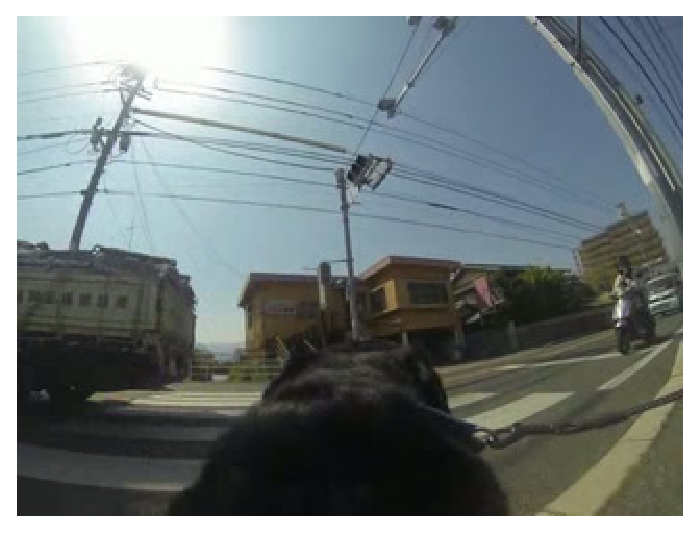
\includegraphics[clip, width=1.7cm]{./Figures/HC005.eps}
          \hspace{0.3cm} { }
        \end{center}
      \end{minipage}
      \begin{minipage}{0.18\hsize}
        \begin{center}
          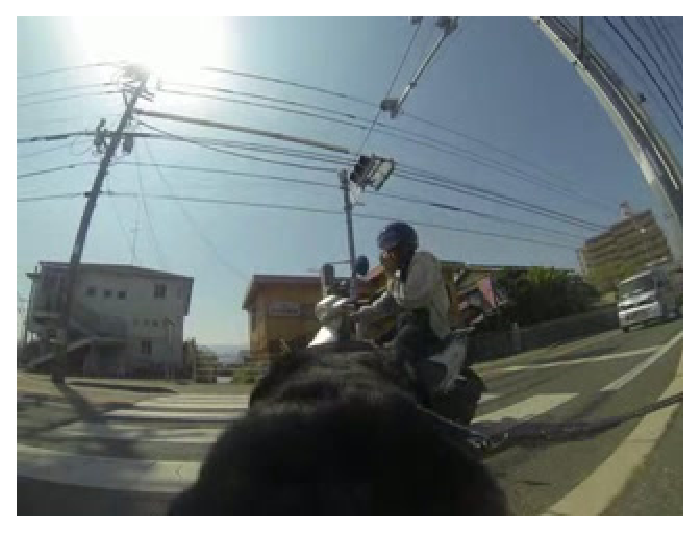
\includegraphics[clip, width=1.7cm]{./Figures/HC006.eps}
          \hspace{0.3cm} { }
        \end{center}
      \end{minipage}

      % 2
      \begin{minipage}{0.18\hsize}
        \begin{center}
          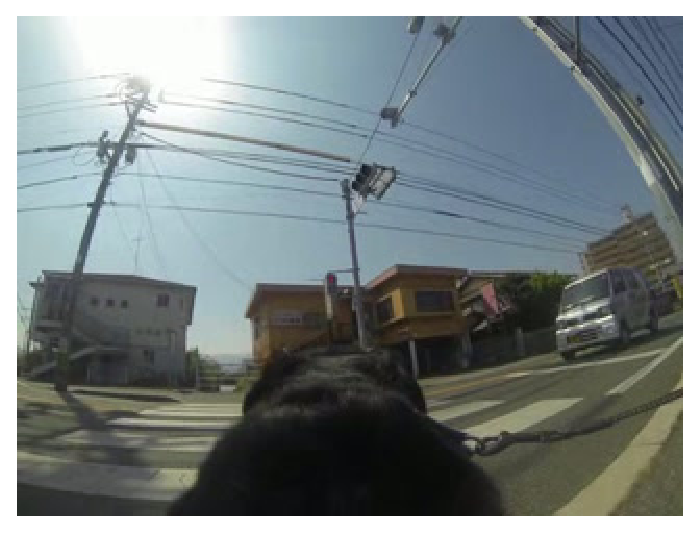
\includegraphics[clip, width=1.7cm]{./Figures/HC007.eps}
          \hspace{0.0cm} {Car}
        \end{center}
      \end{minipage}

      % 4
      \begin{minipage}{0.18\hsize}
        \begin{center}
          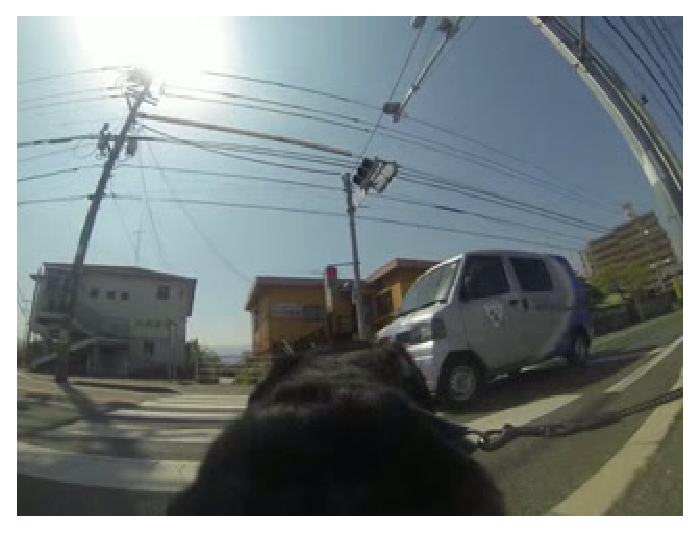
\includegraphics[clip, width=1.7cm]{./Figures/HC008.eps}
          \hspace{0.1cm} { }
        \end{center}
      \end{minipage}
      % 5
      \begin{minipage}{0.18\hsize}
        \begin{center}
          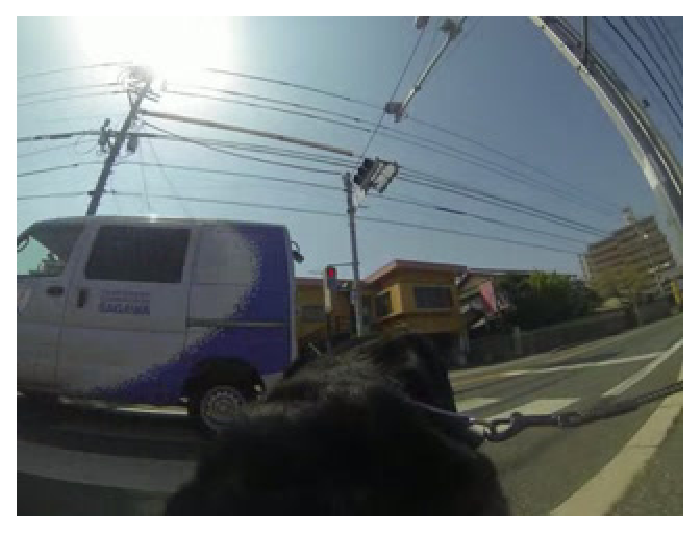
\includegraphics[clip, width=1.7cm]{./Figures/HC009.eps}
          \hspace{0.2cm} { }
        \end{center}
      \end{minipage}
\\
     \begin{minipage}{0.18\hsize}
      \begin{center}
       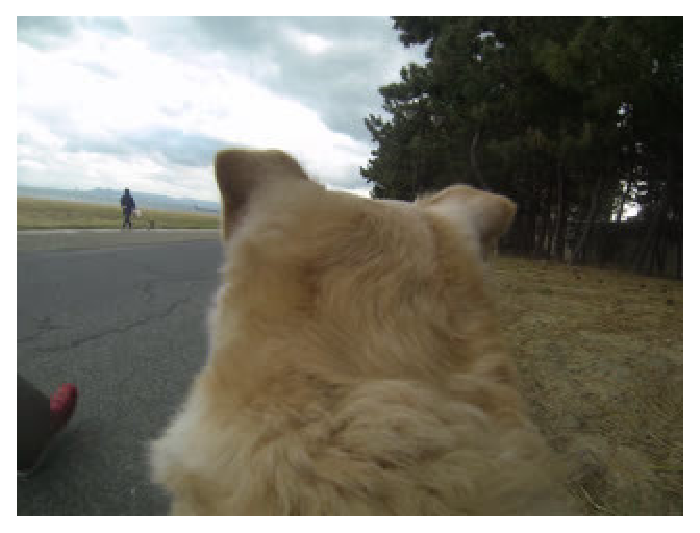
\includegraphics[clip, width=1.7cm]{./Figures/KL001.eps}
       \hspace{0.3cm} { }
      \end{center}
     \end{minipage}
     \begin{minipage}{0.18\hsize}
      \begin{center}
       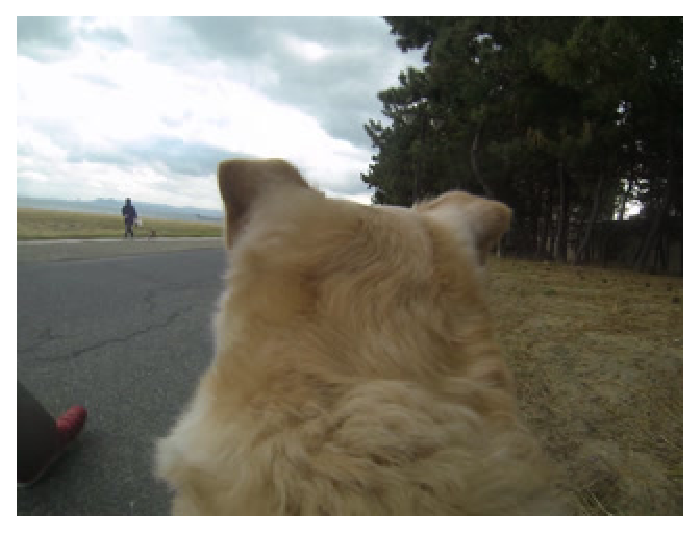
\includegraphics[clip, width=1.7cm]{./Figures/KL002.eps}
       \hspace{0.3cm} { }
      \end{center}
     \end{minipage}
     \begin{minipage}{0.18\hsize}
      \begin{center}
       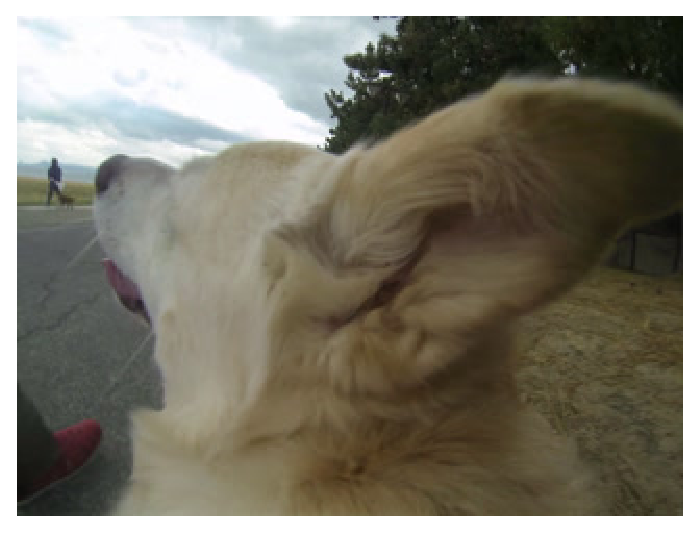
\includegraphics[clip, width=1.7cm]{./Figures/KL003.eps}
       \hspace{0.1cm} {Look\_at\_Left}
      \end{center}
     \end{minipage}
     \begin{minipage}{0.18\hsize}
      \begin{center}
       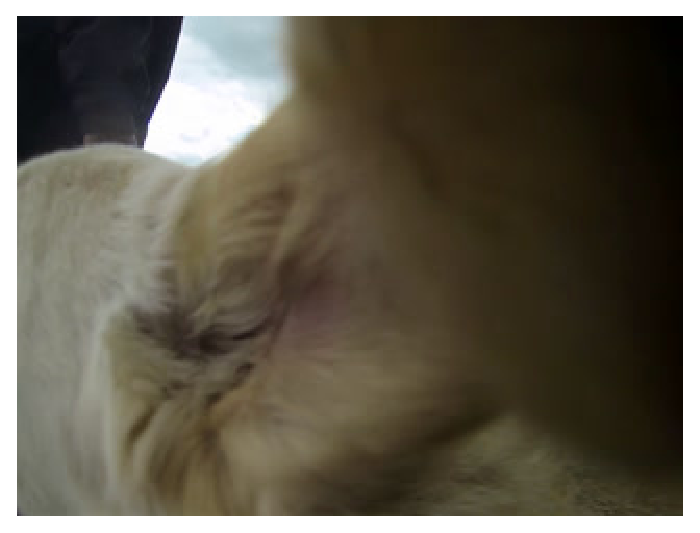
\includegraphics[clip, width=1.7cm]{./Figures/KL004.eps}
       \hspace{1.3cm} { }
      \end{center}
     \end{minipage}
     \begin{minipage}{0.18\hsize}
      \begin{center}
       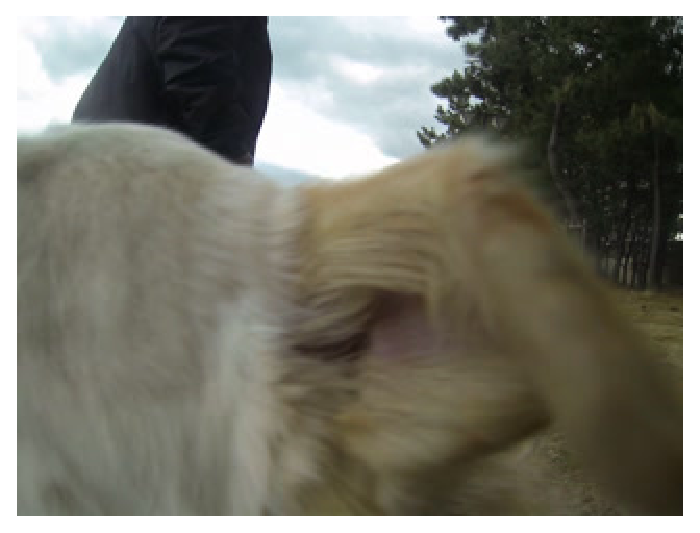
\includegraphics[clip, width=1.7cm]{./Figures/KL005.eps}
       \hspace{1.6cm} { }
      \end{center}
     \end{minipage}

    \end{tabular}
    \caption{DogCentric Activity Dataset}
    \label{DCAD_img}
%  \end{center}
\end{figure}
\section{サイバーレスキュー犬 訓練データセット}
専用の計測スーツを着用した
